% THIS IS SIGPROC-SP.TEX - VERSION 3.1
% WORKS WITH V3.2SP OF ACM_PROC_ARTICLE-SP.CLS
% APRIL 2009
%
% It is an example file showing how to use the 'acm_proc_article-sp.cls' V3.2SP
% LaTeX2e document class file for Conference Proceedings submissions.
% ----------------------------------------------------------------------------------------------------------------
% This .tex file (and associated .cls V3.2SP) *DOES NOT* produce:
%       1) The Permission Statement
%       2) The Conference (location) Info information
%       3) The Copyright Line with ACM data
%       4) Page numbering
% ---------------------------------------------------------------------------------------------------------------
% It is an example which *does* use the .bib file (from which the .bbl file
% is produced).
% REMEMBER HOWEVER: After having produced the .bbl file,
% and prior to final submission,
% you need to 'insert'  your .bbl file into your source .tex file so as to provide
% ONE 'self-contained' source file.
%
% Questions regarding SIGS should be sent to
% Adrienne Griscti ---> griscti@acm.org
%
% Questions/suggestions regarding the guidelines, .tex and .cls files, etc. to
% Gerald Murray ---> murray@hq.acm.org
%
% For tracking purposes - this is V3.1SP - APRIL 2009

\documentclass{acm_proc_article-sp}

%\usepackage[latin1]{inputenc}
\usepackage[utf8]{inputenc}


\usepackage{hyperref}
\usepackage{color}
\usepackage[usenames,dvipsnames,svgnames,table]{xcolor}
\usepackage{listings}


\newcommand{\datatemplate}{
data template
}


\usepackage{Sweave}
\begin{document}
\input{paper-data-restore-model-concordance}

\title{
A Data Restore Model\\
for Reproducibility in Computational Statistics
}
%
% You need the command \numberofauthors to handle the 'placement
% and alignment' of the authors beneath the title.
%
% For aesthetic reasons, we recommend 'three authors at a time'
% i.e. three 'name/affiliation blocks' be placed beneath the title.
%
% NOTE: You are NOT restricted in how many 'rows' of
% "name/affiliations" may appear. We just ask that you restrict
% the number of 'columns' to three.
%
% Because of the available 'opening page real-estate'
% we ask you to refrain from putting more than six authors
% (two rows with three columns) beneath the article title.
% More than six makes the first-page appear very cluttered indeed.
%
% Use the \alignauthor commands to handle the names
% and affiliations for an 'aesthetic maximum' of six authors.
% Add names, affiliations, addresses for
% the seventh etc. author(s) as the argument for the
% \additionalauthors command.
% These 'additional authors' will be output/set for you
% without further effort on your part as the last section in
% the body of your article BEFORE References or any Appendices.

\numberofauthors{3} %  in this sample file, there are a *total*
% of EIGHT authors. SIX appear on the 'first-page' (for formatting
% reasons) and the remaining two appear in the \additionalauthors section.
%
\author{
% You can go ahead and credit any number of authors here,
% e.g. one 'row of three' or two rows (consisting of one row of three
% and a second row of one, two or three).
%
% The command \alignauthor (no curly braces needed) should
% precede each author name, affiliation/snail-mail address and
% e-mail address. Additionally, tag each line of
% affiliation/address with \affaddr, and tag the
% e-mail address with \email.
%
% 1st. author
\alignauthor
Daniel Bahls\\
       \affaddr{Leibniz Information Centre for Economics (ZBW)}\\
       \affaddr{Neuer Jungfernstieg 21}\\
       \affaddr{20354 Hamburg, Germany}\\
       \email{d.bahls@zbw.eu}
% 2nd. author
\alignauthor
Benjamin Zapilko\\
       \affaddr{GESIS - Leibniz Institute for the Social Sciences}\\
       \affaddr{Unter Sachsenhausen 6-8}\\
       \affaddr{50667 Cologne, Germany}\\
       \email{benjamin.zapilko@gesis.org}
% 3rd. author
\alignauthor
Klaus Tochtermann\\
       \affaddr{Leibniz Information Centre for Economics (ZBW)}\\
       \affaddr{D\"usternbrooker Weg 120}\\
       \affaddr{24105 Kiel, Germany}\\
       \email{k.tochtermann@zbw.eu}
}
% There's nothing stopping you putting the seventh, eighth, etc.
% author on the opening page (as the 'third row') but we ask,
% for aesthetic reasons that you place these 'additional authors'
% in the \additional authors block, viz.
%\additionalauthors{Additional authors: John Smith (The Th{\o}rv{\"a}ld Group,
%email: {\texttt{jsmith@affiliation.org}}) and Julius P.~Kumquat
%(The Kumquat Consortium, email: {\texttt{jpkumquat@consortium.net}}).}
\date{14 May 2012}
% Just remember to make sure that the TOTAL number of authors
% is the number that will appear on the first page PLUS the
% number that will appear in the \additionalauthors section.
  
\maketitle



\begin{abstract}


Researchers are more and more requested to publish their scientific data sets for purposes of transparency, re-use, and reproducibility.
Particularly in economics and the social sciences, researchers often use sensitive statistical data that underlie protection policies which inhibit distribution to third party archives.
In addition, a considerable quantity of data sets combines data from one or more external providers, which complicates the setting for curation-related activities. %---when working with data copies
These circumstances give us reason to pursue a \textit{data restore model} on the basis of fine-grained referencing that allows to trace data provenance to the original archive in charge of curation.
%One goal is to enable data publication in difficult cases.
%Moreover, we show how the gaps between data citation and code integration can be closed as to eliminate all manual efforts of arranging code and data for reproduction attempts. 
One goal is to enable data publication in difficult cases, and another one is to show how the gaps between data citation and code integration can be closed in order to eliminate all manual efforts of arranging code and data files for reproduction attempts. 
On this basis we develop the requirements for a data restore model and elaborate a generic design in view of an overall data management infrastructure.
We further explore an experimental implementation which we validate by taking the example of a real-world publication in economics.
Eventually we close with the vision of a \textit{data and code ontology} that carries statistical models from paper to a re-usable semantic level.




\end{abstract}

%todo: categories, keywords, terms setzen
% http://dl.acm.org/ccs_flat.cfm
% http://www.acm.org/about/class/2012

% A category with the (minimum) three required fields
\category{H.3.7}{Digital Libraries}{Miscellaneous}
%A category including the fourth, optional field follows...
\category{I.2.4}{Knowledge Representation Formalisms and Methods}{Semantic networks}

\terms{Design, Algorithms, Economics}

\keywords{Research Data Management, Semantic Digital Data Library, Linked Data, Statistics} % NOT required for Proceedings




\newpage

\section{Introduction}

Repeatability of research results is a fundamental criterion in science. % experiments are conducted in different environments and by different persons as to validate whether the results depend on considered parameters only.
Experiments must lead to the same findings when conducted by other persons or in other environments, under the premise of keeping relevant and considered parameters constant.
% sciencemag article on "Reproducible research in computational science"
In computational research, this remains unverified in many cases due to various reasons \cite{Peng02122011}.
One of them is the plain fact that the supporting data is often unavailable to others which gives rise for a more organized and open data management practice \cite{Wood1298248}.
While a scientific publication is commonly understood as synonymous with a peer-reviewed article alone, program code and data take the role of nice-to-have additional material only that rarely find their way to the public.
%There are numerous examples of research publications that turned out inconsistent eventually, either because of mistakes,  
%There are numerous examples of inconsistent research  that illustrate how 




Transparency and verification of results not only are gestures of good scientific practice but essential if the statements published in the name of science are to reflect profound and solid knowledge.
%BZ: Hier koennte noch der von dir angesprochene punkt zu journals und datenpublikationen hin. Mehr als 1-2 saetze brauchts hier aber nicht.
The problem might be less significant in technical domains where relevant theories and best practices would be validated eventually as soon as they are applied.
Decision makers in public sector and industry, however, often rely on surveys and studies which do not necessarily have to stand proof when made use of. 
The case of a research study on cultural integration of immigrants in the UK  
shows that inconsistencies occur in the social sciences as well.
The data was available to the community \cite{dataset_FNSEM} which allowed other researchers to investigate and after all heavily criticize their publication as its results could not be reproduced \cite{arai2011fragile}.
To underscore their critique, they published the source code of their own analyses online and in this way called for clarification. % and revealed their difficulties in replicating.
The original authors responded with an errata in which they acknowledged the faults.
At the same time, they presented a modified version of the statistical model they had applied and managed to produce the previous findings again while admitting that ``the results are now less clear-cut and [they lost] statistical significance'' \cite{bisin2011errata}.
%
% btw, the paper is not retracted. the authors did not highlight anywhere around the homepage that there was an issue. they simply list the errata as another publication and that's it.
% it has 58 citations as of today, and the errata is not cited once at all.
% ich will hier aber kein aggressives politikum starten, wir wollen ja auch niemanden abschrecken und schreien, dass wir hier aufräumen wollen, oder?
%
 

Data availability was the key for verification in the example above.
Yet, when it comes to analyses and the methods applied, textual reports typically lack many of the algorithmic details needed for reproduction or re-use after all.
Altogether, the media type itself seems rather unsuitable for this purpose, which is why there are many voices in the scientific community promoting the idea of program code to be included as substantial artefacts along with the article.
In this sense, some researchers even view source code as the main contribution.
This viewpoint is often referred to as the \textit{Claerbout principle}:
"An article about computational science in a scientific publication is not the scholarship itself, it is merely advertising of  the scholarship. The actual scholarship is the complete software development environment and the complete set of instructions which generated the figures" \cite{Buckheit1995b} \cite{de2001reproducible}.
In support of this view \cite{KoenkerZeileis2009} investigated reproducibility in econometrics and pointed out how software tools can be used to organize data, code, and documentation in this domain.
As part of a replication study they have also shown that important details are missing in the two example papers examined and filled in the blanks by publishing source code and data of the eventually successful replication attempts.

Both, data and code resources make a valuable contribution if findings are to be reproducible and re-usable in computational research.
And yet, there is more to be considered.
A comprehensive review of the \textit{JMCB\footnote{Journal of Money, Credit, and Banking} data+code archive} revealed that provenance information for the data used is often incomplete and that submitted code does not reproduce the results either \cite{RePEc_ejw_journl_v_4_y_2007_i_3_p_326_337}.
It is not uncommon that even the original authors have difficulties understanding the details of their own work only few months after publishing already.
Apparently, these issues are faced in many other areas of computational research too
% reproducibility is a problem in many domains
% bio informatics (case studies 100 articles..) mit leisch, sweave autor
\cite{hothorn2011case}
% empirical software engineering
\cite{gonzalez2012reproducibility}
% signal processing
\cite{vandewalle2009reproducible}
% ecology
\cite{cassey2006reproducibility}
% "replicating empirical results is an underemphasized, yet essential element of scientific progress."
% Report on the American Economic Review Data Availability Compliance Project
% http://www.aeaweb.org/aer/2011_Data_Compliance_Report.pdf
which can be understood as a problem of insufficient documentation.


With the increasing use of statistics software \cite{RePEc_hum_wpaper_sfb649dp2011_020}
these problems emerge in empirical research in general where more and more statisticians promote the use of literate programming techniques  
% Executable Papers for the R Community: The R2 Platform for Reproducible Research
\cite{leisch2011executable}
% literate statistical practice (reproducibility and documentation)
\cite{rossini2003literate}
%as to combine report text and coding in single executable scripts so that a basic documentation of the analyses is already given naturally.
which combine report text and coding in single executable scripts in a way that clarifies the link between research code, the figures produced, and the findings naturally.
In both of the examples above, the authors made use of the literate programming tool Sweave \cite{lmucs_papers_Leisch_2002} 
so that their reports can be generated again, from data processing to generating the report document, under the premise that the data is given and the system environment allows for correct execution.


%However, 
Empirical research is often based on sensitive data that cannot be shared easily.
%A general solution to this problem is to transform such data sets into anonymized public-use files that can be distributed without infringements of data protection.
One solution to this problem is to transform such data into anonymized public-use files that can be distributed without infringements of data protection.
But doing so requires careful verification in terms of cell sizes and de-anonymization and requires additional efforts, often on the researchers' side.
Moreover, researchers hesitate to publish their own data if incentives are not clear, especially when they had a lot of work producing it.
In addition, data is often obtained from several sources and the mere citation of them does not give any details on the file formats used or way of composition as used as input for the computer program.
%BZ: hier kommst du wieder zurueck zu den daten (wenn auch mit anderem schwerpunkt), nachdem das thema oben eigentlich abgehakt wirkte und du zum thema program code und danach zu provenance gegangen bist. sollte dieser abschnitt ueber sensitive data nicht zu dem data abschnitt weiter oben? gehoert ja irgendwie schon zusammen, oder?


%These circumstances motivate our efforts to elaborate on a holistic solution for the statistical domain that enables the exact reconstruction of individual research data sets as were used by the researchers.
In this paper we aim to overcome these challenges for the domain of statistical data and elaborate on a holistic solution to enable the exact reconstruction of individual research data sets as used originally by a researcher.
We pursue the idea of a \emph{data restore model} that is based on fine-grained data referencing as described in earlier works \cite{BahlsTochtermann_2012}
where further background and motivation is explained more thoroughly.
Since this referencing technique can be viewed as means for precise citation, the linkup to provenance and further documentation on the particular data version is given which again contributes to clarity.
The idea is to equip researchers with means that make full transparency possible even in difficult settings of protected and distributed data sources, so that reconstruction remains a question of access permission only.
The restore model is designed to bridge the gaps between data citation and program code and to seamlessly integrate with preferred research tools, so that no further manual work is required in setting up data and code resources for replication attempts.
Eventually, the goal is to provide researchers with the ability to close all missing links from data sources and processing to figure plotting and report generation as to create trust in their findings which from another perspective could be an incentive to do so.
On the basis of this data restore model, we elaborate the requirements it carries on the entire information infrastructure between researchers, archives, and libraries.


 
The remainder of the paper is structured as follows. 
In Section \ref{sec:relatedwork} we discuss related work relevant to our approach. 
%In section 2 we present a case study with real world examples, where literate programming with research data is applied. 
%Based on these examples we propose a generic data reconstruction model in section 3. 
The requirements for a data restore model are elaborated in Section \ref{sec:datareferencing} by which we develop a generic solution.
An experimental implementation is presented in Section \ref{sec:impl} where we explore its application in context of a case study from economics.
%Finally, we conclude and present future work in Section \ref{sec:outlook}.
Finally, we conclude in Section \ref{sec:outlook} with summary and outlook on future work and present a vision that illustrates the potential of this approach .




\section{Related Work}\label{sec:relatedwork}

%argumentation: our tpoic is related to several fields and tries to connect lose ends. topics: general reproducibility, data access and privacy, data referencing/citation

%------------------------------------
%topic general reproducibility

% stichpunkte, was hier noch rein kann
% da muss man mal sehen, ob das wirklich alles rein muss
The problem of reproducibility in computational research has been addressed by many.
If re-execution of experiments is the goal, it is necessary to capture information on the entire system environment used in order to make sure respective processes can be performed under the same parameters
%
% preservation of digital objects and processes (problems with system environments)
%
%
% Virtual Machines: eine Virtuelle Maschine wird gespeichert (ungefähr die Ecke Andreas Rauber, Klaus Rechert)
% preservation of processes and digital objects
\cite{DBLP_conf_ercimdl_Rauber12}
\cite{Rechert_2010_EBS_1816123_1816182}
.
%\cite{Guttenbrunner_2012_MFE_2180868_2180876}
%This alone is already a very hard problem, because it must include hardware and software dependencies to very detail.
This alone is a very hard problem already, because the chain of dependencies in terms of hardware and software has to be captured and restored to the very detail.
In this regard, \cite{Schwab_2000_MSC_369545_369555} illustrates how the problem of software dependencies for computational research could be solved with the help of build scripts such as make files.
Nevertheless, the achievements in this area seem promising, and the opportunities for application such as  
%
%
% Virtual Research Environments / E-Science, Grid Computing
%
% collage is an executable paper environment to re-run analyses (grid-based)
\cite{Nowakowski2011608} % waren die 2. gewinner der exec paper challenge 11
%
% scientific workflows passen hier auch
are great. % todo: echt beknackte formulierung
%BZ: wie waers mit:
%Nevertheless, the achievements in this area and the opportunities for application such as \cite{Nowakowski2011608} seem promising.
As the goal of our research is to find means for precise reconstruction of data sets and direct integration with program code, these approaches make a good complement. % todo: formulierung   
%BZ: As we aim to find means for precise reconstruction of data sets and direct integration with program code, the approaches complement each other.

Particularly for the domain of empirical research, we found the literate programming approach very appealing as it seems light-weight and suitable for the many, less complex scenarios.
It interweaves source code and text for the report, so that all processing steps are already quite well-documented. 
%Approaches like \cite{lmucs_papers_Leisch_2002} prove that the reproduction of research results is technically feasible, but there are still challenges that hinder this process: 
%Literate programming approaches like Sweave \cite{lmucs_papers_Leisch_2002} or Knitr\footnote{\url{http://yihui.name/knitr/}} are suitable for the reproduction of research results. 
Tools like Sweave \cite{lmucs_papers_Leisch_2002} or Knitr\footnote{\url{http://yihui.name/knitr/}} are already accepted as helpful means to reproduce analyses and document its steps
% Executable Papers for the R Community: The R2 Platform for Reproducible Research
\cite{leisch2011executable}
% quite a number of recent publications make use of them.\footnote{The list of Sweave citations in scientific publications of many areas is increasing continuously.}
% the author's initial motivation was to be able to re-run his own analyses again
%
% literate statistical practice (reproducibility and documentation)
\cite{rossini2003literate}
and therefore suitable for the reproduction of research results. 

%
% weitere evidenzen fuer die beliebtheit als reproduzierbarkeits-tool sozusagen. brauchen wir das?
%
% literate programming for transparency
% Encoding Transparency: Literate Programming and Test Generation for Scientific Function Libraries
%\cite{flood2012encoding}
%
% A Multi-Language Computing Environment for Literate Programming and Reproducible Research
%\cite{Schulte2012}
%
% Literate Spreadsheets (nicht gelesen ;)
%\cite{dinmore2012design}

% noch mehr kram, "Reproducible computational experiments using SCons"
% cite{fomel2007reproducible}




Source code for computational research does not need to be executable in order to make a valuable contribution to transparency
as it is a detailed documentation of the processing and a valuable resource as such, which is part of the argumentation in 
% all these resources should have an identifier, as the title suggests
% they won the executable paper challenge, although it is not executable. it says quite something
%
% verifiable computational research
%
\cite{gavish2011universal}.
The Verifiable Computational Research community aims to collect data, code and intermediate results of research processes as a trace to make findings verifiable.
Their automatic capturing process is integrated with the researchers' workflow, and hence successful as well as unsuccessful attempts can be reviewed eventually. 
%However, the VCR community argues that the source code does not have to be executable, source code as a detailed documentation of the processing suffices, and other intermediate results should be captured, so that the research is tracable and verifiable.
We share their view in a pragmatic sense. The code does not need to be executable, if it is, the better. % todo: formulierung 
%BZ: Ich wurde den letzten teil ab "if it is" einfach streichen...
Either way, source code should be picked up as part of the publication material whenever possible
%
% source code is important 
%
% * for replicability not only data itself, but also program code, e.g. of mathematical calculations, is necessary
%
% science code manifesto
\cite{barnes2012science}\footnote{\url{http://sciencecodemanifesto.org/}}.


%------------------------------------
%topic data access and privacy

%wenn das als related work durchgehen soll brauchen wir hier noch mehr referenzen...

%One of the main problems in empirical research, however, is the fact that a great deal of the data used is sensitive and hence protected.
%Other data sets are used commercially and usage policies prohibit its further distribution
One of the main problems in empirical research, however, is that a large amount of the data used is sensitive and hence protected, or underlies certain usage rights due to commercial use. % REF da gibts bestimmt irgendwas vom RatSWD oder so...
Therefore the problem of data availability cannot be solved as the legal situation simply prohibits the further distribution to other parties.
% open data
But recently, as a result of the Open Data movement a large degree of data sets has been made publicly available by governments, statistics offices and research organizations. This data can be used for research, but is not always citable or referencible in a way it is required for scientific publications like using persistent identifiers. The publictaion of such data as Linked Open Data \footnote{http://linkeddata.org/} allows a precise identification and recerence of single entities such as data sets or particular indicators. Furthermore, by using the Linked Science Ontology \cite{kauppinen_et_al_linked_science_2011} abstract research processes can be modelled and represented. But, this ontology does not address the issues of data access and availability.

%

%

% panton principles
%\cite{murray2010panton}

% CKAN muss auch noch irgendwo rein
% das ist doch aber immer open data.
% wir können es nutzen um die templates zu publizieren, ansonsten kommt es wieder in die rubrik: geht nicht, datenschutz


%
% LOD
%
%  * LOD for scientists.
%
%\cite{Halb_LDOW08}
%
% * Linked Data: dazu sollten wir etwas mehr sagen, aber das hast du ja oben schon etwas ausgeführt
%   knüpft an Metadaten an, Ontologien wie Data Cube etc, semantic Web
%
% da passt auch die linked science ontology
%\cite{kauppinen_et_al_linked_science_2011}


%--- der rdf teil hier kann eigentlich oben mit in die related work oder?

%Represented in RDF, using the RDF Data Cube Vocabulary (QB) for example, documentation on the variables could be interweaved within and machines could make meaning of it too, if given according to established standards like SDMX, DDI or alternative application-oriented ontologies.
%%There are other initiatives that like to see this data in this structure too
%It would integrate with other open government data.
%There is interest from the linked data community as well. \cite{Halb_LDOW08}
%Eventually, RDF provides strong means for referencing as it builds on URIs\footnote{Or IRIs} which allows for decentrally organized ID assignment at no costs. 



% why linked data is not enough for scientists, also reproducibility etc.
%\cite{bechhofer2010linked}

%
% other related work:
%
% * data provenance: können wir anstoßen und sagen, dass wir ja egal was referenzieren
% * genauso auch die Diskussionen um Metadaten: DDI, SDMX, alles in eine Box und sagen, dass wir es hier nicht brauchen
%


% data cite
%\cite{Citation2011}
% SDMX, DDI

%BZ: provenance und metadaten würde ich hier glaub ich rauslassen, das spannt den bogen sonst zu weit. habe auch lod nur kurz mitaufgenommen.



%------------------------------------
%topic data referencing / citation

%Data citations typically point to entire data sets as a whole. 

%BZ: hier könnte eigentlich ein bißchen allgemeinsa zu data referencing / citation hin... das fängt oben schon ein wenig bei open data und lod an. dann könnte man sich im folgenden kapitel nämlich ein wenig kürzer fassen und besser auf das model fokussieren.










\section{The Data Restore Model}\label{sec:datareferencing}

We begin this section by developing the requirements for a data restore model.
Subsequently, we elaborate a generic design and discuss its implication on an overall data mangement infrastructure and the workflows involved.


\subsection{Requirements}\label{sec:req}

In the following, we want to develop the ideas of a referencing technique and take into account the recommendations fromulated by \cite{RePEc_ejw_journl_v_4_y_2007_i_3_p_326_337} which we refer to using parentheses \textit{(A-J)}.
Whichever data management solution is applied eventually should fit to the researchers' workflows and practices in order to be effective and thus accepted \cite{Feijen_2011}.
In the ideal case, researchers can use their preferred tools with no further hassle preparing anything at the time of data submission.
%  (assisting tools to reduce efforts)
%
%On the side of reuse, there should not be any unnecessary efforts in re-using these resources either, meaning that no puzzling and manual tinkering in organizing data and code to make it run.
On the side of reuse, there should not be any efforts in composing and organizing these resources either, meaning that no puzzling and manual tinkering in organizing data and code is required to make it run \textit{(F partly)}.
Location and structure of data files on the local file system should be inherently specified, so that it integrates perfectly with the code.
\footnote{In this regard, software and system specifications are as important. This kind of documentation can be organized independent of the issues addressed in this paper, we therefore do not further address it here.}
  
There are plenty of prevailing file formats, ranging from CSV, XML, Excel, entire RDBMS dumps to specific software-dependent and even unknown individual ``raw" types of formats.
McCullough et al. recommend the use of ASCII encoding \textit{(D)} for the benefit of re-usability, we therefore want to exclude binary formats from our discussion.
As to be less restrictive and support more contemporary encodings such as UTF-8, we want to pursue the idea of self-describing documents with information on its own encoding contained.\footnote{Otherwise, data would need to be converted back and forth which causes trouble whenever a character has no representation in the ASCII standard}
A format-independent solution should be found whereas most importantly, any restored data set must equal the original as to perfectly integrate with the code in the end \textit{(E)}. 
% which gives us a clear (requirement for successful) test case
Thus, we note that data citation by persistent identifier (as is the current practice in data publishing) is not sufficient for this purpose, since these identifiers point to data sets on a more abstract level only and do not distinguish or specify a particular format.
\footnote{Most data agencies offer download in various formats while the content is filed under the same persistent identifier.}

  
Further, the data restore model should be applicable for protected data as well \textit{(supports G)}.
This might sound surprising to the reader as sensitive data cannot be shared per se and a restore concept appears redundant.
Nevertheless, we want to make the point that the spectrum from open to closed data is gradual, since some data is access-restricted only and can be obtained under certain policies and regulations.
Whether or not a data set can be handed out should be a question on legal level only, the restore technique itself, however, should cater for these cases as to give means for repeatability in every scenario.
% später nochmal aufgreifen: meta data von protected data sharen. man kann wenigstens herausfinden, dass es diese daten gibt

Either way, pointers to the provenance of data should be available that give documentation and further background such as contact information for any version being used.
While new persistent identifiers are commonly given for major data updates and releases only, those versions with minor bug-fixes cannot be referred to with precision so far.\footnote{Surely, an author can give a note on the time of data download or acquisition in the paper. This is rarely practiced, and data reconstruction in this case again involves vagueness and human efforts.}
%A common practice is to assign new persistent identifiers to major data updates while those versions with minor bug-fixes cannot be referred to so far.\footnote{Surely, an author can give a note on the time of data download or acquisition in the paper. This is rarely practiced, and data reconstruction in this case again involves vagueness and human efforts.}
%It is also to consider that new persistent identifiers are given for major data updates only while those versions with minor bug-fixes cannot be referred to with precision so far.\footnote{Surely, an author can give a note on the time of data download or acquisition in the paper. This is rarely practiced, and data reconstruction in this case again involves vagueness and human efforts.}
The use of versioning systems could help identify individual releases at detailed level \cite{KoenkerZeileis2009} which should integrate seamlessly with the data restore model.
Eventually, references to service points providing this information should be given along with the submission material.
This could further be realized with Web Services that accept requests for information or data content on a technically fully supported level, so that up-to-date user assistance can be provided directly within the tools used in a research environment \textit{(B)}.
Depending on regulations, the actual data content identified by a given model instance could be transferred on request, possibly using authentication mechanisms, so that the data set can be restored locally using the original data sources.
\footnote{Authentication can be realized using SSL for example. If transfer via internet is considered too insecure, the API can be used to collect data requests as such and to initiate the procedure according to the respective policies.}


In contrast to the copy-based approach, the referencing technique allows data and documentation to be maintained at one responsible archive only, with the result that no duplicate efforts have to be made in terms of data curation which is particularly relevant in cases where (several) external sources were used.
This improves quality of service as all enquiries about data can be answered with the highest possible level of expertise available and gives a clear view on responsibilities in addition.

As a result of this discussion we formulate the following requirements for the data restore model:



\begin{enumerate}\label{reqlist}
	
%  \item First and foremost, data sets should be reconstructable to the fullest, so that experiments can be repeated with the exact same data.
%  \item \textbf{Equality:} Data sets should be reconstructable to the fullest, so that experiments can be repeated with the exact same data.
  \item \textbf{Equality:} A data file restored by the model must equal its original on character level\footnote{Depending on character encoding and operating system, the files may differ on bitstream level while the textual content is equal.}, so that it integrates perfectly with the software and program code used by the researcher.
  
%  \item The technique must be applicable to protected or closed data as well.
  \item \textbf{Protection:} The model must be applicable for protected data (closed data) as well, in strict accordance with secured protection.
 
%  \item \textbf{Curation:} The technique makes possible that data could be maintained and curated at those archives only that are responsible of maintenance with the required level of expertise.
%  \item \textbf{Curation:} The technique makes possible that data maintenance and curation needs to be done for the original copy only, right at the responsible archive, whereas harvesting techniques work efficiently 
  \item \textbf{Curation:} Using the model, data maintenance and curation needs to be done for the original copy only, right at the responsible archive, whereas documentation can be distributed efficiently on the basis of harvesting techniques.

  
  % das ist vielleicht etwas hart formuliert
%  \item Researchers are not disturbed by the introduction of technical hinderances such as new data formats or other obligations.
%  \item \textbf{Usability:} The method should integrate seamlessly with the researchers' workflows and suit to their preferred data formats. 
%  \item \textbf{Usability:} The method should integrate seamlessly with the researchers' workflows and comply with their preferred data formats. 
  \item \textbf{Usability:} The method should integrate seamlessly with the researchers' workflows and comply with their preferred tools. 
		% It should be independent of any particular data format. % kann man das so reinschreiben, klingt jedenfalls komisch
  
  % auch soll es möglichst einfach auf neue unbekannte Datenformate anwendbar sein, mitunter um zukunftsfähig zu sein
  \item \textbf{Formats:} The method should be sustainable and applicable to common, alternative, unknown and future data formats.

  % verwendung von ids macht das ganze glasklar. kann man als argument gegenueber query-approach anbringen, wenn wir wollen 
%  \item It should be simple and transparent, so that problems can be traced easily. % mit hilfe der direkten pointer ist alles gestochen scharf und einfach zu debuggen (?)
%  \item \textbf{Tracability:} The technique itself must be transparent, so that problems can be traced and questions can be answered efficiently.
  \item \textbf{Traceability:} The technique itself must be traceable, so that references to data content can be followed efficiently, by humans and machines.
 %wenn du mit traceable meinst, dass zb berechnungen auf den daten nachvollziehbar sein sollen, dann wuerde ich hier auf jeden fall die ids nennen. transparent ist hier dann als begriff zu allgemein.
 
%  \item overall, it has to meet the constraints and requirements from all parties involved in the overall data management infrastructure, such as archives, researchers and libraries. % was vergessen? und not openly available data = closed data? 

  \item \textbf{API:} The data restore model should include pointers to Web Services that provide documentation, contact information or, if applicable, the actual data content upon request.

\end{enumerate}




%------------model--------
\subsection{Designing the model}
%\subsection{ID-per-Value Approach}


The requirements can be realized in several ways.
However, giving freedom to researchers to use or reuse data in their preferred environments and associated formats needs careful consideration.
Data could be offered in a variety of formats, each version provided with means for persistent identification, so that data citation as well as seamless code integration is ensured.
But this approach requires program code to function on complete data sets, which impairs usability considering that researchers typically select slices of indicators and observations\footnote{e.g. selection of certain indicators and reference periods from large time series data} for input to their programs.
Further, the approach would lead to multiple persistent identifiers for content-wise identical data and complicate bibliometric measures.
These conditions suggest the use of a primary data representation from which all other formats can be derived whereas one referencing method only is needed to serve all scenarios.
As a consequence, such model must give means for identification of any possible data slice from global scope.
Pointers to respective repositories in combination with structured queries (such as SQL or SPARQL) could be a solution.
A challenge in this approach, however, is that such queries produce result sets in the shape of tables which yet need to be transformed into this unspecified format as used by a researcher.
In the following, we elaborate a model that aims to overcome these challenges.

The model has to make sure that individual data slices and values can be identified without ambiguity in the long term.
As we could not find an established data model for statistical data that is not subject to change and incorporates versioning at the same time, we discarded model-based queries and decided to use individual identifiers for every single value of a data set.
The number of IDs needed is certainly high and questions of scalability raise immediately.
On the other side, the IDs we are going to introduce can as well be interpreted as single-result queries or as the variables of a regular query.
%To give an estimation on the technical implications, the number of additional triples needed is twice the number of data values, or the same number only if not linked with other semantic resources.
%Maintenance could be supported with tools and there should not be any additional efforts, provided that the data is maintained in a structured representation already.
%BZ: what tools?
However, we would like to have a discussion on this na\"{\i}ve approach and leave the investigation of scalability for now.
We will introduce the concept of a \textit{data template} which is based on the idea to replace every value within a data file with its associated ID, so that the original file can be restored again simply by replacing them back with its associated values.
This could also help solve some of the problems in using linked data for scientific purposes \cite{bechhofer2010linked}\footnote{The problem of precise data references has been recognized by the Semantic Statistics community as well \url{http://datalift.org/en/event/semstats2013}.}, which will be the basis of the model.


With the ongoing linked open data movement, awareness and knowledge about semantic technologies and the RDF data model has found its way to many application domains, among which the domain of statistical data\cite{Halb_LDOW08}.
%BZ: Hier suche ich noch ein, zwei Referenzen raus, die zusammen mit Halb_LDOW08 aufgezaehlt werden koennen.
These technologies break down the separation between black box data bundles and attached metadata as they interweave data with its documentation.
%BZ: These technologies break not only down the separation between black box data bundles (the raw data) and attached metadata as it interweaves data with its documentation.
%BZ: They also enable the publication, sharing and interlinking of data.
The data content is more accessible and interpretable to machines which sets the stage for a variety of new applications, e.g. for data retrieval \cite{BahlsTochtermann_2012}.
%BZ: das wesentliche fuer unseren approach ist hier eigentlich gesagt, alles andere wuerde wohl eher in die related work passen, oder? wuerde diesen absatz mit dem folgenden zusammenfassen.







\subsection{Workflows}

% edawax survey sven vlaeminck
%
%\cite{LQURN:NBN:NL:UI:10-1-114595}
%

If implemented in big scale as a holistic information infrastructure for research data management in statistics, the presented approach has further implications on workflows and gives ideas for a big picture.
Data archives could offer the download of data templates along with the actual data, so that researchers have the precise references right from the beginning of their research.
Alternatively, researchers could pull the data on the basis of these data templates alone from within their research tool, provided that a respective plugin is available.
The advantage in the latter case is that this procedure could be embedded within their program code and no further modifications on data and code need to be done at the time of publishing.
The researcher simply submits code and data templates, and other researchers can rerun the same analysis without any manual arrangements or collection of resources, simply by executing the code.


In case the researcher used own data, the data would have to be submitted to an affiliated archive\footnote{Researchers have to archive their data, either locally or at another archive. By "affiliated archive" we denote this repository.} in beforehand where the respective data template and IDs involved are generated first.
The archive returns the template to the researcher who can then publish it in the same way as described above.
This procedure must be supported with tools for mapping and ID generation.
Furthermore, these tools should provide for further semantic annotation of the content (using the RDF Data Cube Vocabulary for example) so that documentation about the data is available as well.
Figure \ref{fig:modelprocessing} outlines the overall process.


%Figure \ref{fig:modelprocessing} outlines the overall process and suggests roles and responsibilities for archives and digital libraries.
%The data itself would be maintained at the archives where Web Services provide access to up-to-date information and, if the policies allow, to its contents.
%Data templates and source code resources behind a scientific article could be maintained at the library


\begin{figure}[htb]
\centering
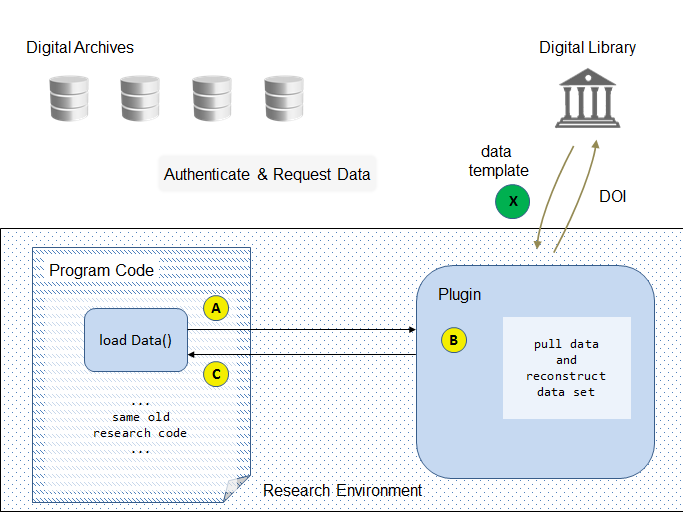
\includegraphics[width=.48\textwidth]{img/fig-model-processing.png}
\caption{
Using the data restore model
}
\label{fig:modelprocessing}
\end{figure}


%BZ: die ersten beiden absaetze klingen sehr hypothetisch und zeigen eher verschiedene szenarien einer nutzung auf, wenn ich das richtig verstehe. ich wuerde in dem abschnitt glaub ich nur die grafik zeigen und anhand dieser dann einen konkreten ablauf darstellen (mit teilen aus den ersten beiden abschnitten). klar ist das dann in gewisser hinsicht auch hypothetisch, aber wenn die grafik zuerst kommt, viel anschaulicher.



























%\section{A case study - Two real world examples}
%\section{An example from the economics}\label{sec:impl}
\section{Experimental Implementation}\label{sec:impl}

%We have implemented
In this section, we present a prototype implementation of the data restore model and a plugin called \textit{ddocks}\footnote{\textit{ddocks} is short for \textit{data docks} which is meant to reflect the ``transshipment" character of the interface between data retrieval and processing.} 
for the computing environment R.
Since literate programming already is a prominent approach to replicability in the computational statistics community \cite{leisch2011executable} (particularly supports recommendation \textit{(A)}) we want to demonstrate how the plugin can further strengthen this concept.
%We begin with the creation of data templates and IDs using two data sets from the sources of our example paper \cite{KoenkerZeileis2009}.
%The plugin implementation is explained subsequently, and we close this section with a validation that tests reconstructed and original data files for equality.


In the following, we explain the concept of data templates by taking the example of two data sets from the sources of \cite{KoenkerZeileis2009}. 
%The \textit{ddocks} plugin and a basic validation which are part of the Sweave sources for this article.
A description of the \textit{ddocks} plugin implementation follows thereafter,
and a basic validation is given at the end of this section which we have incorporated as part of the Sweave sources for the article the reader is currently looking at.
The source code is available on GitHub, and respective links are given at the bottom of each subsection.



\subsection{Generating the Data Templates}

%We introduce the concept of a \textit{data template} which is based on the idea to replace every value within a data file with its associated ID, so that the original file can be restored again simply by replacing them back with its associated values which solves the requirements of \textit{Equality}.
The data template contains a header section in which we can specify encoding and tokens that are used to identify IDs within the template.
In addition, we also declare Web Service addresses for every namespace used (which is only one for our example) under the pragmatic assumption that every namespace can be associated with one archive providing one such Web Service for data enquiries.
%At this point, we do not want to elaborate on the Web Service interface, however, we have used SPARQL endpoints in the proof of concept implementation presented in Section \ref{sec:impl}.


We used a simple script that scans any given input text file for contained values using a regular expression which was specially designed for the data of our example.
For every identified value a static counter variable increments by one which is used to generate the value ID.
We could have used the plain counter value as such, but we decided to hash it only to highlight that these IDs need no meaningful structure at all.
In combination with the examplary archive namespace \textit{http://demoarchive.demo/data/} we obtain full URIs for all values, making them referenceable worldwide from any context.
To obtain the \textit{body} of a data template, all values are replaced with their abbreviated URIs and surrounded with angle brackets for parsing purposes.
A \textit{header} section is prepended to this part which we start with an XML-like notation that declares character encoding and \textit{ddocks} version as to give basic information about how to interpret the contents of this file.
The \textit{ddocks-header} tag opens the actual header section in which the namespaces used are listed with their associated URI prefix and repository API for which the prototype expects the address of a SPARQL endpoint.
It further declares the parse tokens used to identify IDs in the template body, so that clashes with format-specific syntax can be avoided.
Eventually, we append the body section right after the newline character behind the close tag of the header section to complete the data template.
Figure \ref{fig:datatemplate} shows an excerpt from one of the two data templates we have created.



\begin{figure*}[htb]
\centering
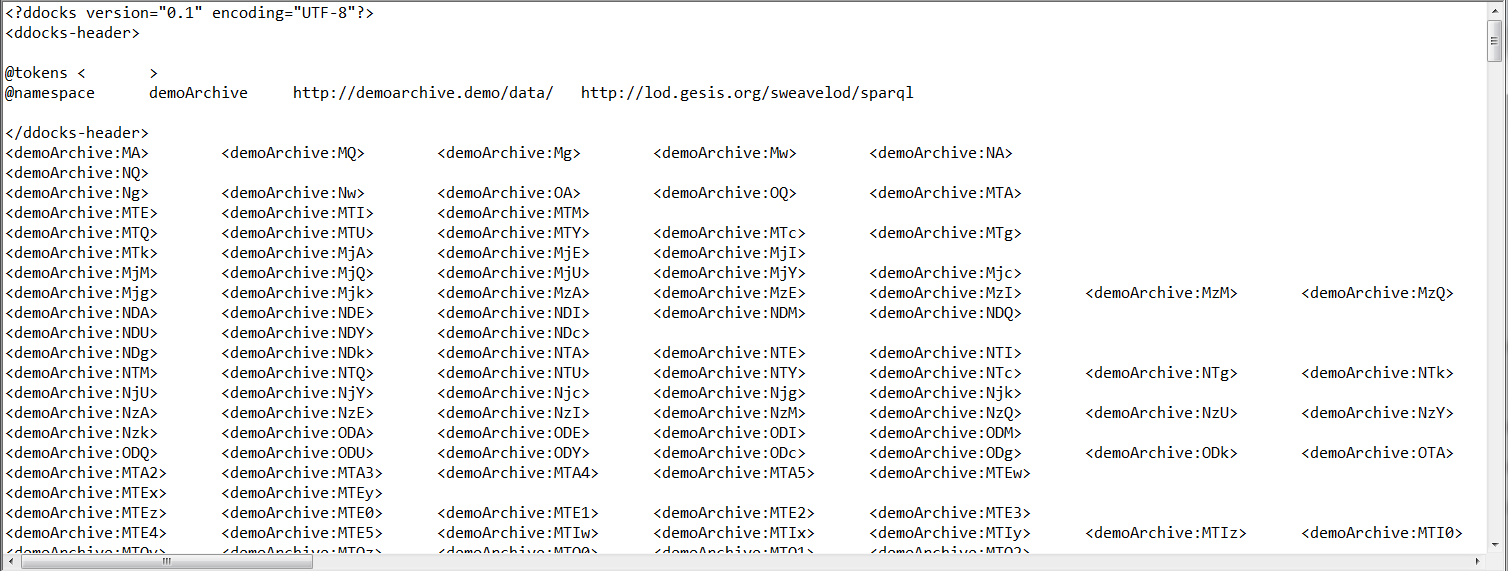
\includegraphics[width=.95\textwidth]{img/datatemplate.png}
\caption{
%Excerpt from one of the data templates
%Data template excerpt from one of the data templates
Data template for one of the two data sets (\textit{rk.raw})
}
\label{fig:datatemplate}
\end{figure*}


The script also produces an RDF document that contains the mapping from the URIs to their associated values.
The simple ontology behind consists of one class only (\textit{DataReference}) and all its instances (value IDs) map to a literal (value) using the \textit{rdf:value} relation.
Finally, we added these triples to an experimental triple store at GESIS that is presently open to the public.
Please note that no further semantics were modelled as we wanted to demonstrate the minimal efforts necessary to follow the presented approach.

%
% link to source code
%
\url{https://github.com/dbahls/ddocks-utils.git}



\subsection{The R-Plugin}


The signature of \textit{ddocks\_restore}, the only function offered by the plugin, expects two parameters.
The first parameter is a connection object from which the data template will be read.
The second parameter specifies the target file the restored content will be saved to.

First, \textit{ddocks} interprets the information given in the header.
Using the declared open and close tokens, it collects all IDs occurring in the template body and organizes them by namespace which is the key to identify the respective data repository.
Iterating over these namespaces, the values are queried from the associated SPARQL endpoint\footnote{This is done in bundles so as not to query every single value separately. Then again, as to avoid oversized queries, these bundles are limited to a number of 30 IDs per query.}
and replace the IDs in the template body which is then written to the target file.



We run this procedure for the two data templates we have generated earlier
\begin{Schunk}
\begin{Sinput}
R> ddocks_restore(
+    file("./data-templates/data.dj.ddocks"), 
+    targetfile="data.dj")
\end{Sinput}
\end{Schunk}

\begin{Schunk}
\begin{Sinput}
R> ddocks_restore(
+    file("./data-templates/rk.raw.ddocks"), 
+    targetfile="rk.raw")
\end{Sinput}
\end{Schunk}
and reproduce the data files on the local file system.
\textit{ddocks} takes these files as a cache and skips when the restore command is run again, so that the data does not have to be reconstructed every time the code is executed.
%Researchers could embed these calls within their source code to load the data by template at the beginning of their analyses and leave it there without being bothered.
Researchers could embed these calls within their source code to load the data by template at the beginning of their analyses without being bothered again, and no further modifications are needed at the time of publishing.


%
% link to source code
%
\url{https://github.com/dbahls/ddocks.git}




\subsection{Validation}


We validate this experimental implementation with respect to the requirements developed in Section \ref{sec:req}.
As this approach is based on URIs, namespaces can be used to identify archives, and in combination with locally organized IDs every single value of any data set can be referenced from any context (\textit{Traceability}).
The requirement item \textit{Curation} is addressed as well, because data can be referenced with precision and maintenance of every data can be done in one place. 
Since the use of RDF allows us to add an additional link between ID and value, we can separate the two and disclose all information about the data in very detail in machine-understandable form, and yet protect the values (\textit{Protection}).
Furthermore, when every value can be referred to from anywhere, a simple technique can be applied to enable format-independent reconstruction of data files for which we introduced the concept of a \textit{data template}.
Particularly the document-specific declaration of tokens enables a format-independent solution (\textit{Formats}) as this flexibility allows us to avoid syntactical clashes with the particular data format used.
We have used SPARQL endpoints as a generic implementation of the \textit{API} which only served for the purpose of data retrieval.
For actual application, a more elaborated API should be developed that could be based on Web Services.



Eventually, we have to show that the restored files equal their originals on character level (\textit{Equality}).
If the two expressions
\begin{Schunk}
\begin{Sinput}
R> all.equal(
+    readLines("data.dj"), 
+    readLines("koenker-zeileis-09/data.dj")) 
\end{Sinput}
\begin{Soutput}
[1] TRUE
\end{Soutput}
\begin{Sinput}
R> all.equal(
+    readLines("rk.raw"), 
+    readLines("koenker-zeileis-09/rk.raw")) 
\end{Sinput}
\begin{Soutput}
[1] TRUE
\end{Soutput}
\end{Schunk}
evaluate to TRUE we have successfully validated the approach in terms of functionality.

We also inserted the two restore calls above in the source code of our example paper (\cite{KoenkerZeileis2009}) right before the load-data calls respectively, and running Sweave on it produced a report identical to the published article.\footnote{using R x64 2.15.3 on Windows}


%
% link to source code
%
\url{https://github.com/dbahls/paper-restore-model.git}


\section{Summary, Vision and Outlook}\label{sec:outlook}


The ideas presented in this work can be used to offer data and code behind research publications, which increases transparency, re-use, and reproducibility.
We have formulated requirements on the basis of the recommendations in \cite{RePEc_ejw_journl_v_4_y_2007_i_3_p_326_337} and further followed the idea of fine-grained data referencing in our data restore model.
%Within the data template single data values can be addressed, even if the original data set is not publicly available.
The introduced concept of data templates uses precise pointers to the original data sources and can be disseminated freely as they do not disclose sensitive content.
Since data files can be restored in the format used by the researcher, the template technique closes the gaps between data citation and program code integration.
The \textit{ddocks} prototype illustrates how the restore model can be applied in a way that enables a "one-click" solution for re-running analyses on other systems provided that users have permission to acquire the data and system dependencies are resolved.
Especially if linked with research articles, the resources can be used in tutorials to teach computational research in practice, serve as re-usable research resources, or can be used within review-processes.
With the precise identification of values, data provenance can be clarified comprehensively whereas responsibilities for maintenance and documentation of a data set are left to one archive respectively, so that harvesting techniques can be used efficiently to carry forward documentation, notes and updates about the data.



Assigning URIs to single data values sets the stage for integration with RDF which has potential for valuable applications.
A semantic model could offer researchers to run same analyses on updated data with no efforts on data retrieval and composition.
While most statistical models today exist on paper only, the current work on reproducibility allows to rerun it again on the original or updated data, and the vision is to make them re-usable for other data as well.
A research publication could remain more relevant for extended periods of time if its predictive model on time series data for example can still be used on new records while the specific results of a published article may no longer be relevant to the community.
Linked with thesauri, researchers could find these models by topic and re-use them in their own context while valuable user assistance can be given automatically if the semantic annotations specify clearly the kind of data it can process meaningfully.


Moreover, these models could serve as an input for the artificial intelligence community as they often describe measures for abstract concepts like \textit{living standards} or \textit{justice} which are typically hard to model.
Although these models are and should always be debatable, the semantic linkage to statistical indicators gives information on aspects that are relevant for understanding these concepts.
Further, predictive models could be combined in ensembles trained with machine learning techniques to further increase accuracy, which might again serve the computational statistics community in their research.


Considering the coupling of data or data references with code and the report text of a research publication eventually, the idea of a \textit{data and code ontology} comes up that models the interconnection between data, code and research results in detail. 
Moreover, it could also be used to model algorithmic transitions from original to intermediate and result data sets, which would help clarify data provenance and allow for reproduction from open intermediate data sets while original data might be closed an unaccessible.
We want to explore this scenario on the basis of \cite{arai2011fragile} for which Sweave sources are available while the data set is access-restricted.
Yet, scalability remains to be tested in regard to curation efforts and technical performance.
We will investigate the design and development of a data and code ontology in future work for which we take into account recommendation \textit{(C)} in \cite{RePEc_ejw_journl_v_4_y_2007_i_3_p_326_337} and other
%
% recommendations (liste von ressourcen, die gegeben sein sollten, damit reproduktion möglich ist)
%
\cite{KoenkerZeileis2009} 
% haben wir oben schon erwähnt
% mccullough, got replicability
%\cite{RePEc_ejw_journl_v_4_y_2007_i_3_p_326_337}
%
% further guidelines
\cite{baiocchi2007reproducible}
%
% Gentleman: "important, if not essential, to integrate the computations and code used in data analyses,...."
\cite{gentleman2007statistical}
%
% Reporting guidelines for simulation-based research in social sciences
\cite{rahmandad2012reporting}
for the purpose of replicability in computational research.
% Replication attempts and intermediate results should be incorporated in an ontology as well
% these outcomes can be linked and support the linked science ontology etc.
% VCR, point (J) in mccullough


%
% Zudem könnte man versuchen obige guidelines noch weiter ausbauen und folgendes mit aufnehmen
%
%  * Spezifikation von Systemumgebungen - Anknüpfung an Rauber, 
%  * Maven, RPM, dependency management
%  * Replikationsversuche (steht schon in den guides)
%



%
%
% cleanups for a camera-ready version:
%
% * intro, erster absatz: discipline-specific solutions are needed
%
% * outlook: data and code ontology, wie sieht es aus mit den Verifiable Computational Research resourcen, replication attempt und linked science ontology?
%
% * Bibliography: unvollständige Angaben: De Leeuw, Barnes
%
% * id-approach: we should also mention: path-based approach: id-per observation + predicate-path to value, lower number of ids required, but maybe not precise enough? other difficulties then, but needs to be explored too (outlook/design)
%
%








\balancecolumns


\bibliographystyle{abbrv}
\bibliography{bibliography}


 

\end{document}

